\documentclass{report}
\usepackage[utf8]{inputenc}
\usepackage{amsmath}
\usepackage{graphicx}
\graphicspath{ {./images/} }

\title{Approfondissements en mathématiques : cours 1ère}
\author{Marin Recopé de Tilly Blaru}
\date{Année scolaire 2021/2022}

\renewcommand*\contentsname{Sommaire}

\renewcommand*\chaptername{Chapitre}

\begin{document}


\maketitle

\vspace{5mm}

\tableofcontents

\newpage

\chapter{Introduction aux Mathématiques}

\section{Un tout indivisible}
Les mathématiques sont des processus qui permettent de relier des idées abstraites. Une idée abstraite est une idée qui a différentes représentations matérialisables sans être elle même matérialisable, par exemple le chiffre 3, des couleurs... \\ \\
Les raisonnements mathématiques ne sont pas linéaires, il faut faire attention à ne pas cloisonner ses connaissances. \\
\emph{nb} : La gestion des fichiers en informatique est totalement linéaire. Pour résoudre ce problème, il existe des logiciels comme Obsidian.

\section{Les mathématiques, une science infinie ?}
En 1900, les mathématiciens se rencontrent à Paris. Un des plus connus, Lagrange, énumère alors les problèmes du millénaires : selon lui il en existe 10. Lagrange proclame que si ces problèmes sont résolus, les mathématiques seront alors "finies".  \\ \\
Gödel, un mathématicien allemand, va alors chercher à démontrer le contraire. Il écrit alors le théorème d'incomplétude de Gödel. Ce dernier dit que si une théorie se suffit à elle même, alors elle est fausse. \\ \\
Pour l'anecdote, quiconque résout l'un des 10 problèmes de Lagrange gagne 10 millions d'euros. Le dernier problème à avoir été résolu : la conjecture de Poincaré en 2003.


\chapter{Le repère cartésien}

\section{Descartes}
Descartes est un mathémathicien français du XVIe siècle. C'est lui qui a inventé le premier repère dans la géométrie, qu'on appelle donc "repère cartésien". Il a donc été le premier à lier géométrie et algèbre, tout en modernisant les vecteurs. 

\section{Introduction au repère cartésien et à ses avantages}
Un repère cartésien associe à tout plan P
    \begin{math}
        \rightarrow \mathbb{R}^2 = \mathbb{R} \times \mathbb{R} = \left \{(x, y), x, y \in \mathbb{R} \right \} 
    \end{math}
    et 
    \begin{math}
         M \rightarrow (x, y)
    \end{math} \\
Le repère présente de nombreux avantages : \begin{itemize}
    \item Très efficace pour l'étude de situations de parallélisme ou d'intersection.
    \item Gère très bien les translations 
\end{itemize}

\section{Les inconvénients du repère cartésien}

Le repère cartésien présente néanmoins de nombreux inconvénients comme celui de ne pas très bien gérer les rotations.

\subsection{Exemple d'un inconvénient : le cercle}
Pour les droites, on a facilement $y = ax + b$ mais pour le cercle (tous les points alignés à la même distance d'un point que l'on appelle centre du cercle), c'est plus difficile. \\ \\
On cherche l'équation cartésienne d'un cercle en plusieurs étapes. \\
Avec $P$ le plan, $\Omega$le centre du cercle, $C$ le cercle et $M$ un point du cercle. On a dans $P$ : 
$(\Omega,r) = \left\{ M \in P \; / \; \|\Omega \vec M \| = r \right\}$ et on considère dans $P$ : $\Omega (x\Omega ; y\Omega)$ et $r \in \mathbb{R}^{*+}$ avec soit $M(x ; y) \in P)$. \\

\textbf{1/ Écrire en fonction de $x$ et de $y$ le réel $\| \Omega \vec M \|$} \\
Dans $R$, nous avons : 
\begin{align}
    \Omega \vec M \binom{x - x\Omega}{y - y\Omega} \Rightarrow \|\Omega \vec M \| = \sqrt {(x - x\Omega)² + (y-y\Omega)²}
\end{align}

\textbf{2/ En déduire que :} \\
\begin{align}
    M(x;y) \in C(\Omega;r) \Leftrightarrow \|\Omega \vec M\| &= r \\ \sqrt {(x-x\Omega)² + (y-y\Omega)²} &= r \\  (x-x\Omega)² + (y-y\Omega)² &= r² 
\end{align}


\subsection{Repères alternatifs}
Il existe donc des repères alternatifs avec par exemple des repère à coordonnées polaires tels que : $P \rightarrow \R^2 \text{et} M \rightarrow (rayon;angle)$. \\
Ainsi pour un cercle, on a  : 
\begin{gather}
    (x-1)^2 (y-1)^2 = 1 \quad \text{coordonnées cartésiennes } \\ r=1 \quad \text{coordonées polaires}
\end{gather}


\chapter{Démontrer que $(x^n)' = nx^{n-1}$ : généralisation de la 1ère et 3ème identité remarquable}

\emph{À la base, on souhaitait démontrer $(x^n)' = x^{n-1}$ (voir plus loin) mais on devait d’abord généraliser la première est la troisième identité remarquable.}

\section{Introduction au coefficiant binomial et à la factorielle}

Pour comprendre ce chapitre, nous avons besoin de comprendre certaines notions. 

\subsection{Factorielle}
La factorielle de $n$ se note $n!$. Pour comprendre la factorielle, rien de mieux qu'un exemple : 
\begin{gather}
    4! = 1x2x3x4
\end{gather}
Par convention, la factorielle de 0 est égal à 1 et la factorielle de 1 est égal à 1. 

\subsection{Coefficient binomial}
Le coefficient se note $C_n^k$. Il est égal à : \begin{gather}
    C_n^k = \frac{n!}{k!(n-k)!}
\end{gather}
La notation anglophone du coefficient binomial est $\binom{n}{k}$

\section{Généralisation de la première et troisième identité remarquable}

\subsection{Généralisation de la première identité remarquable}
Pour $n \in \N \; \; et \; \; \forall(x,y) \in \R^2$, on a :
\begin{gather}
    (x+y)^n = \sum_{k=0}^n C_n^k x^k y^{n-k}
\end{gather}

\subsection{Généralisation de la troisième identité remarquable}
Pour $\forall n \in \N^* \; \; et \; \;\forall (x,y) \in \R^2$, on a :
\begin{gather}
    x^{n+1} - y^{n+1} = (x-y) \times \sum_{k=0}^n x^k y^{n-k}
\end{gather}

\emph{Exemples}
\begin{align} 
    x^2 - y^2 = x^{1+1} - y^{1+1} 
    &= (x-y)\sum_{k=0}^1 x^k y^{1-k} \\ 
    &= (x-y)(x^0y^{1-0}+x^1+y^{1-1}) \\ 
    &= (x-y)(x+y)
\end{align}

\begin{align} 
    x^6-y^6 
    &= (x-y)(x^0y^5+x^1y^4+x^2y^3+x^3y^2+x^4y^1+x^5y^0) \\ 
    &= (x-y)(y^5+xy^4+x^2y^3+x^3y^2+x^4y+x^5) \\ &= (x-y) \sum_{k=0}^5 x^k y^{5-k} 
\end{align}

On rappelle que $\sum_{k=0}^5 k$ est la notation de la somme.

\section{Résolution du problème}
Soit $n \in \N^{*}$
\begin{gather}
    \forall x \in \R \; ; \; f_n = x^n
\end{gather}
Soit $a \in \R$
\begin{gather}
    \lim_{h \to 0} \frac {f_n(a+h) - f_n(a)} {h} \; = \; \lim_{h \to 0} \frac {(a+h)^n - a^n} {h}
\end{gather}

Grâce aux généralisation des premières et troisièmes identités remarquables (voir juste au dessus), l’on peut continuer cette démonstration :
\begin{align} 
    \lim_{h \to 0} \frac {(a+h)^n - a^n} {h} 
    &= \lim_{h \to 0} \frac {(a+h-a) \sum_{k=0}^{n-1} (a+h)^k a^{n-1-k} } {h} \\ &= \lim_{h \to 0} \sum_{k=0}^{n-1} (a+h)^k a^{n-1-k} \\ 
    &= \lim_{h \to 0} \sum_{k=0}^{n-1} a^k a^{n-1-k} \\ 
    &= \lim_{h \to 0} \sum_{k=0}^{n-1} a^{k+n-1-k} \\ 
    &= \lim_{h \to 0}  \sum_{k=0}^{n-1} a^{n-1} \\ 
    &= \underbrace{a^{n-1}+a^{n-1}+a^{n-1}+ \cdots + a^{n-1} }_{n fois} \\ 
    &= na^{n-1} 
\end{align}  

On peut donc en conclure que $\forall x \in \R, \; (x^n)' = nx^{n-1}$


\chapter{Triangle de Pascal et lien avec le coefficient binomial}

\section{Introduction}
Voici le triangle de Pascal. On a abordé ce qu'était $C_n^k$ dans le dernier chapitre. 

\begin{figure}[htp]
    \centering
    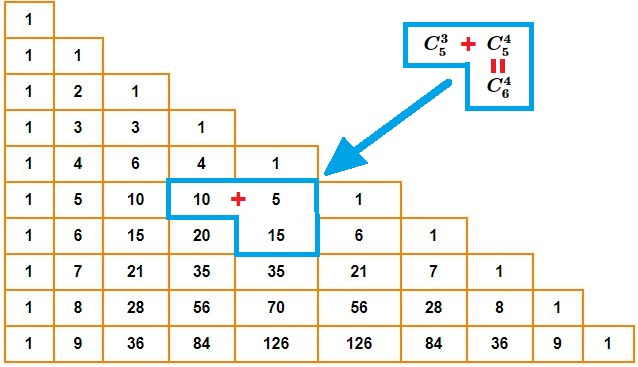
\includegraphics[width=\textwidth]{pascal.jpg}
    \caption{Triangle de Pascal}
    \label{Triangle de Pascal}
\end{figure}

On remarque que si on fait la somme de chaque ligne, on obtient toujours $2^n$ avec $n$ le numéro de la ligne. (Les lignes commencent à zéro). Prenons l’exemple de la deuxième ligne. On a $1 + 2 +1 = 4$ ce qui équivaut à $2^2 = 4$. On a donc : $\sum_{k=0}^n C_n^k = 2^n$. Démontrons le : 

\textbf{Démonstration de $\sum_{k=0}^n C_n^k = 2^n$}
On sait que pour $\forall n \in \N, \; \forall(x,y) \in \R^2$, on a : 
\begin{gather}
    (x+y)^n = \sum_{k=0}^n C_n^k x^k y^{n-k}
\end{gather}
En particulier si $x=y=1$, on a donc avec $n \in \N$ :
\begin{gather}
     (1+1)^n = \sum_{k=0}^n C_n^k \underbrace{1^k 1^{n-k}}_{1} \\
     2^n = \sum_{k=0}^n C_n^k 
\end{gather}

\section{Propriétés}
\begin{itemize}
    \item $\forall n \in \N \; , \; C_n^0 = C_n^n = 1$
    \item $\forall n \in \N, \; \forall k \in [\![ 0;n]\!], \; C_n^k = C_n^{n-k} $ (Cette relation gère la symétrie du triangle de Pascal).
    \item $\forall n \in \N, \; \forall k \in [\![0;n]\!], \; C_n^k + C_n^{k+1} = C_{n+1}^{k+1}$
\end{itemize}


\chapter{Introduction aux probabilités et aux expériences aléatoires}
Pour une probabilité, il faut du hasard, un univers et un événement. Il existe deux types d’expériences aléatoire :

\begin{itemize}
    \item Les expériences aléatoires finies. L’univers $\Omega$ contient un nombre fini. On s’intéresse à ce type d’expérience dans notre scolarité.
    \item Les expériences aléatoires infinies. L’univers $\Omega$ contient un nombre infini.
\end{itemize}
Avant de continuer, il faut mettre au clair certains définitions :

\section{Définitions}

\subsection{Cardinal}
\underline{Cardinal} : soit $E$ un ensemble fini et $E = \underbrace{\{n_1, n_2, \dots \}}_{n \; éléments}$, alors le cardinal de $E$ noté $\#E$ (notation anglaise) ou $Card(E)$ (notation française) équivaut à $Card(e) = n$.

\subsection{Probabilité}
\underline{Probabilité} : Soit $E$ une expérience aléatoire telle que son univers $\Omega$ soit fini avec $\# \Omega = n \in \N$. On appelle probabilité d’un événement $A \subset \Omega$, la fréquence d’apparition d’e l’événement $A$ lorsque $E$ est répété un très grand nombre de fois. Cette quantité est théorique. La probabilité est notée $P(A) \in [0;1]$

\subsection{Variables aléatoires}
\underline{Variable aléatoire} : Soit $E$ un expérience aléatoire avec $\Omega $ son univers tel que #$\Omega = n \in \N$. Toute fonction du type $X : \Omega \rightarrow \R$ est dite une V.A (variable aléatoire).

\subsection{Schéma de Bernoulli}
On considère une expérience aléatoire $E$ d’univers $\Omega_E = \{A,A'\}$. \\
L’arbre de probabilité est :

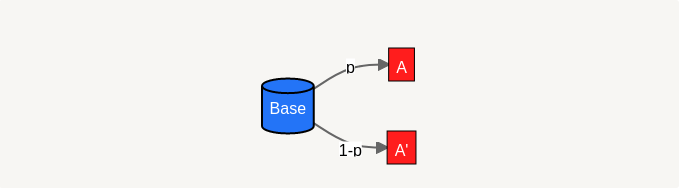
\includegraphics[width=\textwidth]{schema_bernouilli_1.png}
Avec donc $P(A) = p$  et $P(A')=1-p$ \\ \\
On appelle alors un schéma de Bernoulli de paramètres $p$  et $n$ ($p \in [0;1]$ et $n \in \N^*$) noté $B(n;p)$ l’expérience aléatoire qui consiste à répéter $E$ $n$ fois ($p$ étant la probabilité).

\emph{Exemple :} \\
Prenons $E$ = tirer à pile ou face \\
L’expérience $E'$ qui consiste à répéter $E$ n fois est un schéma de Bernouilli. L’expérience $E'$représenté par l’arbre de probabilité suivant est notée $E' \sim B(3;0,5)$

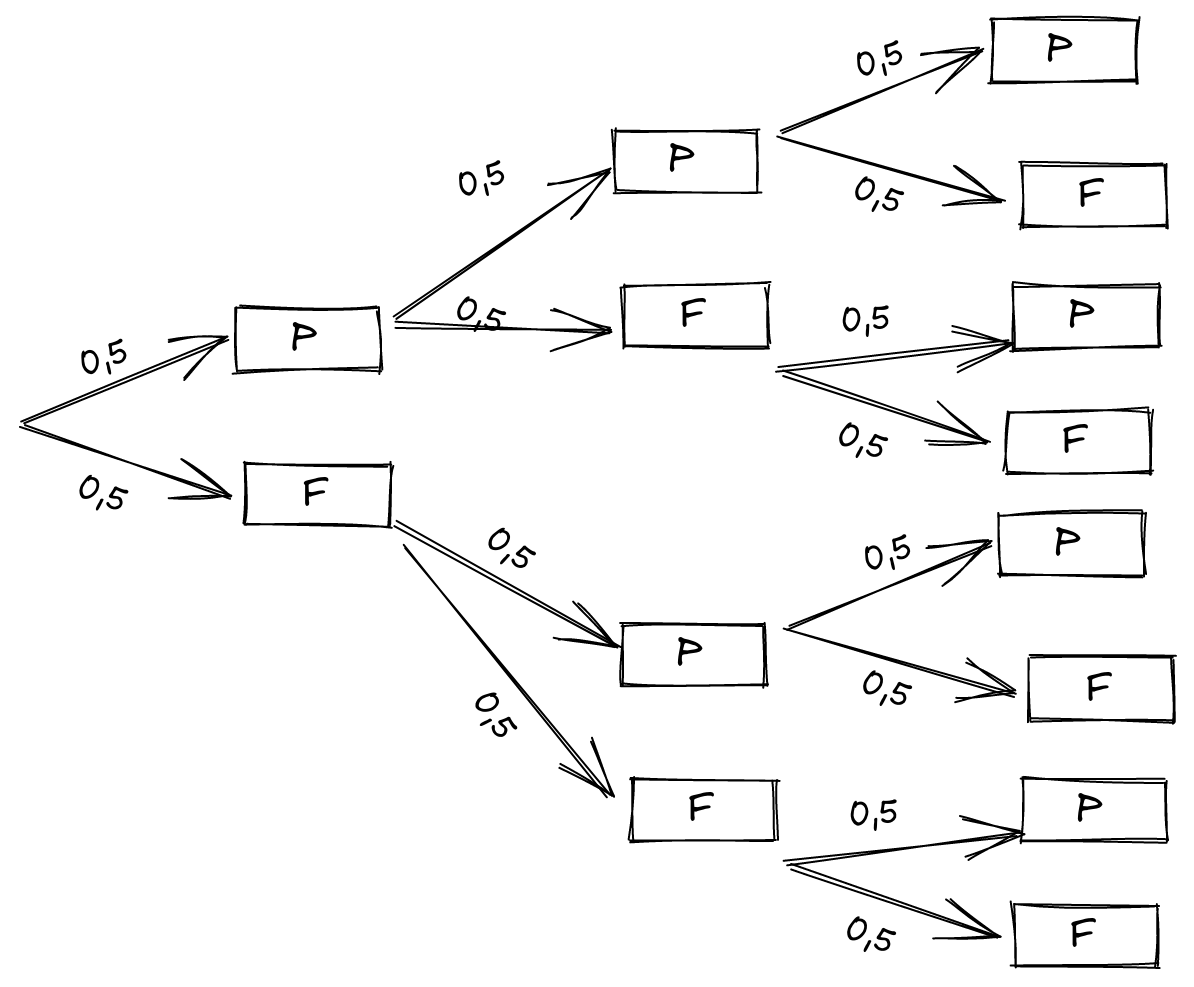
\includegraphics[width=\textwidth]{schema_bernouilli_2.jpg}

Pour résumer l’épreuve de Bernoulli consiste à répéter un certain nombres de fois une situation avec une issue binaire.

\section{Lien entre probabilités et binôme de Newton}
On définit une variable aléatoire $X : \Omega \rightarrow \N$ et on l’associe à l’expérience $E$ comme le nombre de succès constatés. L’expérience $E$ consiste à tirer à pile ou face trois fois de suite. \\
Donc $E \sim B(3;0,5)$. \\
On considère que le succès $S$ est d’avoir pile. 
\begin{figure}[htp]
    \centering
    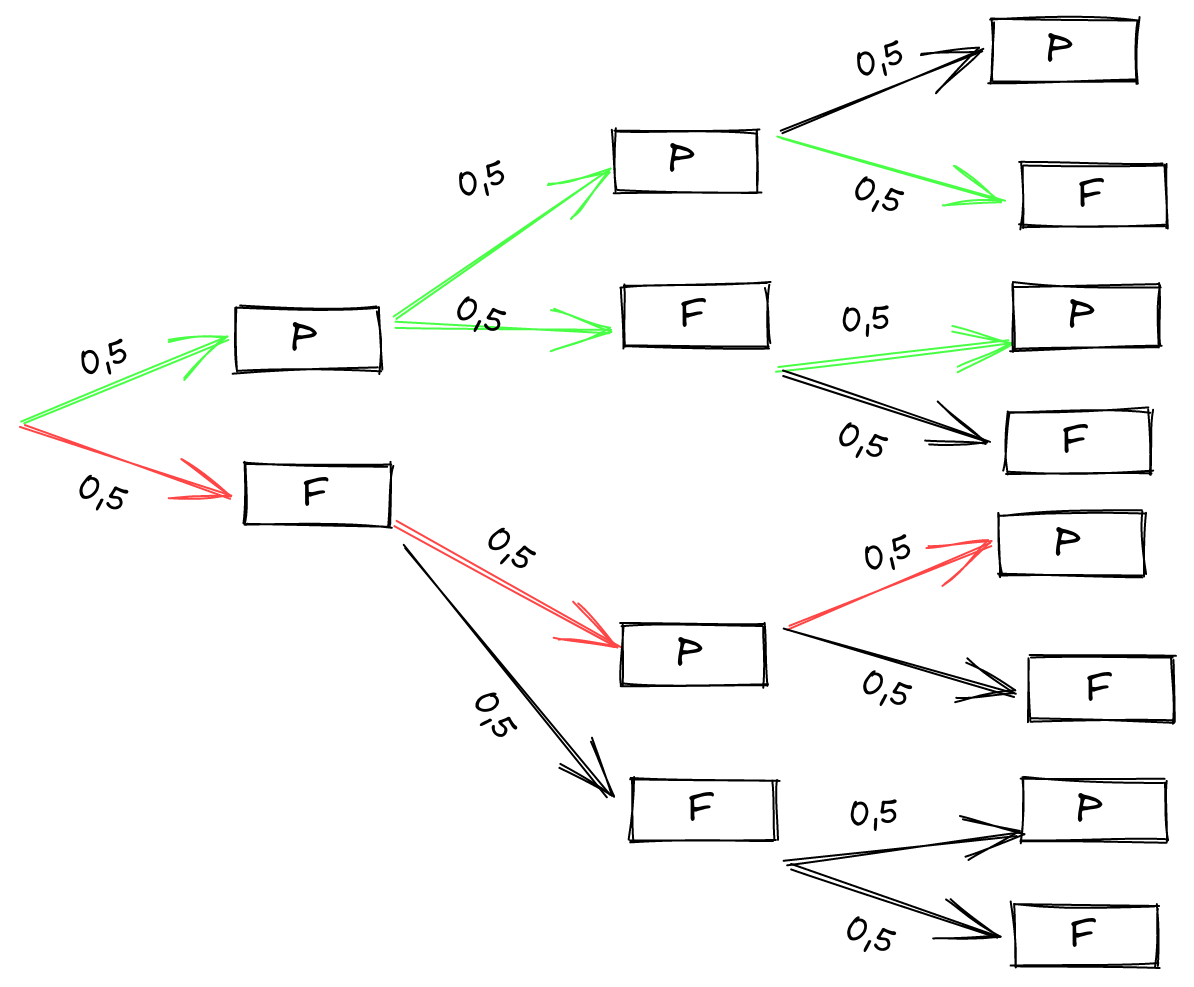
\includegraphics[width=\textwidth]{proba_newton.jpg}
    \caption{Arbre de probabilité de l'expérience E}
    \label{Arbre de probabilité de l'expérience E}
\end{figure} 
On considère le chemin rouge comme l’événement $A \subset E$ et $X : \Omega \rightarrow [\![0;3]\!]$ la variable aléatoire de chaque événement $A$. \\
Alors $A = (F;P;P)$ et $X(A) = 2$ (chances d’avoir $P$ donc que $E$ soit un succès).
De plus, $P(X(A)=2) = \frac{3}{8}$. Ce sont les chemins verts et rouges. \\
Par ailleurs, l’univers $\Omega_E = \{(P;P;P);(P;P;F);\dots)$. \\ 

\textbf{\underline{Théorème}} : \\

Soit $k \in [\![0;n]\!] $ et $n$ le nombre de répétitions de l’expérience et $p$ et $n$ les paramètres de $B(n,p)$. Alors $P(X(A)=k) = C^k_n p^k(1-p)^{n-k}$. 


\chapter{Théories des ensembles}
Nicolas Bourbaki est un pseudonyme utilisé par 8 mathématiciens de l’École Normale Supérieur Ulm. Ces derniers se sont mis en tête dans l’entre deux guerre (années 1930) d’uniformiser les connaissances mathématiques, jusqu’à là très asymétriques en fonction des continents et lieux. \\ \\
Ils vont donc rédiger un ouvrage sous le nom de Nicolas Bourbaki nommé Éléments de Mathématiques qui reprend toutes les connaissances mathématiques de l’époque en onze tomes. \\ \\
Le premier tome s’intitule Théorie des Ensembles car toutes les mathématiques découlent de cette dernière. Nous allons voir partiellement en quoi elle consiste.

\section{Les bases}

\underline{Ensemble} : Un ensemble $E$ est une collection d’éléments qui ont un point commun. \\ \\
\textbf{\underline{Axiome}} : \quad \textbf{L'ensemble vide} \\
Il existe un ensemble noté $\emptyset$ qui ne contient rien. \\ \\
\textbf{\underline{Définitions}} \\
Soient $E$ un ensemble quelconque et $A, B \subset E$, on a :
\begin{itemize}
    \item $A \setminus B = \{ x \in E \; / \; x\in A \; \;  et \; \;  x \notin B \}$
    \item $\overline{A} = \{ x \in E \; / \; x \notin A \}$
    \item $A = B \Leftrightarrow A \subset B \; \; et \; \; B \subset A$
    \item $A \subset B \Leftrightarrow \forall x \in E \; ; \; (x \in A \Rightarrow x \in B)$
    \item $A = B \Leftrightarrow (x \in A \Leftrightarrow x \in B)$
\end{itemize} \\ \\
\underline{Notation} \\
Soit $E$ un ensemble quelconque. Pour tout ensemble $A \subset E$, on note $E \setminus A = \overline{A}$. \\

\emph{Exercice} : Soit Soit $E$ un ensemble quelconque et $A,B \subset E$. Et soit $x \in E$. Montrez les égalités suivantes : 
\begin{enumerate}
    \item $\overline{(\overline{A})} = A$
        \begin{gather}
            x \in \overline{(\overline{A})} \Leftrightarrow x \notin \overline{A} \Leftrightarrow A
        \end{gather} \\
        Donc on a $\overline{(\overline{A})} = A$
    \item $\overline{A \cup B} = \overline{A} \cap \overline{B}$ \\ 
        Tout d’abord montrons que \begin{math}
            \overline{A \cup B} \subset \overline{A} \cap \overline{B}
        \end{math} \\ 
        Cela revient à montrer que $x \in \overline{A \cup B} \Rightarrow x \in \overline{A} \cap \overline{B} $ 
        \begin{gather}
            x \in \overline{A \cup B} \\ \Rightarrow x \notin A \cup B  \\ \Rightarrow  x \notin A \; \; et \; \; x \notin B \\ \Rightarrow x \in \overline{A} \; \; et \; \; x \in \overline{B} \\ \Rightarrow x \in \overline{A} \cap \overline{B}
        \end{gather}
        Pour montrer que $\overline{A} \cap \overline{B} \subset \overline{A \cup B}$, on a juste à faire le chemin inverse de la démonstration.
        Donc $\overline{A \cup B} = \overline{A} \cap \overline{B}$ car $\overline{A} \cap \overline{B} \subset \overline{A \cup B}$ et $\overline{A \cup B}  \subset \overline{A} \cap \overline{B}$
    \item $\overline{A \cap B} = \overline{A} \cup \overline{B}$
        \begin{gather}
            x \in \overline{A \cap B} \\ \Rightarrow x \notin A \cap B \\ \Rightarrow x \notin A \; \; ou \; \; x \notin B \\ \Rightarrow x \in \overline{A} \; \; ou \; \; x \in \overline{B} \\ \Rightarrow \overline{A} \cup \overline{B}
        \end{gather}
        Donc $\overline{A \cap B} = \overline{A} \cup \overline{B}$
    \item $A = (A \setminus B) \cup (B \cap B)$ \\
        À vous de jouer ;)
    \item $(A \setminus B) \cap (A \cap B) = \emptyset$ \\
        À vous de jouer ;)
\end{enumerate}

\section{Produit cartésien d'ensembles}
\textbf{\underline{Définition}} : \quad \textbf{Produit cartésien} \\
Soient $A$ et $E$ deux ensembles quelconques. Alors on définit le produit cartésien de $E$ et de $F$ par : 
\begin{gather}
    E \times F = \{(x,y) / x \in E ; \; y \in F \}
\end{gather}

\textbf{Généralisation} : \\
Soit $n \in \N^* ; \forall i \in [\![1;n]\!]$ et soit $E $ un ensemble quelconque. On a : 
\begin{gather}
    \prod_{i=1}^{n} E_i = E_1 \times E_2 \times E_3 \times \dots \times E_n = \{ \underset{n-uptet}{(x_1; \dots ;x_n)} \; / \; \forall i \in [\![ 1; n ]\!] \; ; \; x_i \in E_i \}
\end{gather}

\textit{Exemple} : \\
$E=\{1;2\}$ et $F=\{a;b;c\}$ 
\begin{enumerate}
    \item Déterminer $E \times F$ et $F \times E$ 
        \begin{gather}
            E \times F = \{(1,a);(1,b);(1,c);(2,a);(2,b);(2,c)\} \\ 
            F \times F = \{(a,1);(a,2);(b,1);(b,2);(b,3) \}
        \end{gather}
    \item Que remarque-t-on ? \\
        Le produit cartésien n’est pas commutatif. 
\end{enumerate}


\section{Cardinaux d'ensembles}

\textbf{\underline{Théorème}} : \quad \textbf{Principes additifs et multiplicatifs} 
\begin{enumerate}
    \item Soit $E$ un ensemble quelconque. Soient $A_1,     A_2, \dots, A_n$ dans des sous ensembles de $E$     deux à deux disjoints. Alors on a : 
        \begin{gather}
            Card(A_1 \cup A_2 \dots \cup A_n) = \sum_{i=1}^{n} Card(A_i)
        \end{gather}
    \item Soient $A_1, \dots, A_n $ des ensembles           quelconques
        \begin{gather}
            Card ( \prod_{i=1}^{n} A_i) = \prod_{i=1}^{n} Card (A_i)
        \end{gather}
\end{enumerate} 

\chapter{Bonus}

\section{Les barycentres}
Un barycentre est un point d’équilibre.  \\

\noindent \underline{Point pondéré} : Un barycentre est un point d’équilibre. \\

\noindent \underline{Barycentre} : Soit $F=\{(A,\alpha_1);(A_2,\alpha_2);\dots;(A_n;\alpha_n)\}$ une famille de points pondérés du plan avec $\forall i \in [\![1;n]\!] ; A_i \in P \; \text{et} \; \alpha_i \in \R $. Alors on appelle barycentre de $F$ le point $G$ du plan $P $ tel que : 
\begin{gather}
    \sum_{i=1}^{n} \alpha_i \overrightarrow{GA}_i = \overrightarrow{0}
\end{gather}
et on le note : 
\begin{gather}
    G = bar(\begin{array}{l|c|r} \rm A & \rm B & \rm C \\ \hline \alpha & \beta & \gamma \end{array})
\end{gather}
De plus, si $\alpha_1 = \alpha_2 = \dots = \alpha_n$, on dit que $G$ est un isobarycentre.

\chapter{Contribuer}

Vous pouvez améliorer ce cours en contribuant à https://github.com/wshchocolatine/math-app

\end{document}
